%% ------------- English version ---------------
\documentclass[english,hidelinks]{sbrt}
\usepackage{newtxtext}
\usepackage[english]{babel}
\usepackage[utf8]{inputenc}
\newtheorem{theorem}{Theorem}
%% ---------------------------------------------
\setlength{\marginparwidth}{2cm}
\usepackage{todonotes}
\newcommand\rigel[1]{\todo[color=green, inline]{\textbf{Rigel}: #1}}
\usepackage{orcidlink}
\usepackage{graphicx}
\usepackage{hyperref}
\usepackage[
  compatibility=false,
  font=footnotesize,
  labelsep=period,
  format=plain,
  justification=raggedright,
  singlelinecheck=false
]{caption}

\begin{document}

\title{Low-Cost Embedded System for Beehive Monitoring}

\author{Igor Costa, Jorge Alves, Ian Dias and Davi Ito
  \thanks{The authors are with Ibmec, Rio de Janeiro, RJ, Brazil.
  E-mails: igorcosta.silva10a@gmail.com,
  jorgedocruzeiro07@gmail.com,
  iandpcarvalho@gmail.com,
  cdavi8249@gmail.com.}%
  }

\maketitle

\markboth{XLIV BRAZILIAN SYMPOSIUM ON TELECOMMUNICATIONS AND SIGNAL PROCESSING - SBrT 2026, SEPTEMBER 29TH TO OCTOBER 2ND, 2026, SALVADOR, BA}{}

\begin{abstract}
Many apiaries have neither mains power nor network coverage, and hive inspections disturb the colony. This paper presents a low-cost ESP32 station, designed for solar power, that photographs a beehive entrance every 10~s with an OV2640 camera and logs the temperature inside and outside the hive on a microSD card, stamped by a DS3231 clock. A YOLO11n detector counts the visible bees. On 3230 hand-labelled frames from three public hives it never saw, it reached an F1-score of 0.83 and a count error of 2.1 bees per frame; on test videos, it reached 0.88 against 0.31 for background subtraction.
\end{abstract}
\begin{keywords}
Beehive monitoring, embedded systems, Internet of Things, computer vision.
\end{keywords}

\section{Introduction}

Bees play a central role in natural and agricultural ecosystems, since their pollination supports the reproduction of flowering plants and the production of crops. The western honey bee (\textit{Apis mellifera}) is among the most widespread crop pollinators, and bee populations face habitat loss, invasive species, emerging diseases, pesticides, and climate change. These pressures call for reliable observation of colony activity over time rather than through isolated inspections \cite{hung2018pollinators,brown2009conservation}.

Traditional inspections are intermittent, require human presence, and disturb the colony each time the hive is opened. Embedded systems are computing platforms built for specific functions under constraints of power, size, and cost, and Internet of Things (IoT) architectures connect them to networks and data services \cite{demicco2020embedded,ray2018iotarchitectures}. This foundation motivates a low-cost, non-invasive station that collects visual and environmental measurements for later analysis.

\textit{Related work.} Zheng et al. combined temperature and humidity sensors inside and around the hive with a webcam at the entrance, and their YOLOv5 and DeepSORT tracker reached 83.5\% MOTA and 77.3\% MOTP at up to 16 frames per second. Narcia-Macias et al. reported 96.28\% tracking accuracy and an F1-score of 0.8319 for pollen detection with the low-cost, YOLOv7-tiny-based IntelliBeeHive, whose \textit{Varroa} detection remains a proof of concept for lack of data \cite{zheng2024intelligent,narciamacias2024intellibeehive}. Henry et al. recorded temperature, humidity, and sound inside hives with a wireless sensor network, which depends on a network that many apiaries lack \cite{henry2019precision}. Tu et al. counted bees at the entrance with background subtraction on a Raspberry Pi and reported an $R^2$ of 0.987 for the count against manual annotations, although illumination, camera placement, and overlapping bees affected the result \cite{tu2016automatic}. Sledevi\v{c} and Matuzevi\v{c}ius published 7200 frames from eight hives, filmed with a smartphone 30~cm above the landing boards at 1920 by 1080 pixels, with every bee labelled by hand \cite{sledevic2024dataset}, and on this material Sledevi\v{c} et al. reached 98\% mean precision in bee detection with YOLOv8m \cite{sledevic2025behavior}. Both studies use smartphone footage, and neither measures how a camera of the class found in low-cost embedded stations affects the detection.

This work proposes a station that records the entrance activity and the temperature of a beehive without opening it and without a network. A camera photographs the entrance on a fixed schedule, two sensors read the temperature inside and the temperature and humidity outside, and both streams reach a memory card stamped by the same clock. Offline, a detector counts the bees in view in each photo, next to the temperature of the same time. With no hive available, the detector is evaluated against the hand labels of Sledevi\v{c} and Matuzevi\v{c}ius on three test hives it never saw in training and compared with background subtraction, and the schedule is set on their hand-labelled footage. The station counts bees in view and claims nothing about pollen, \textit{Varroa}, the queen, or swarming. Counting entries and exits would require tracking each bee through video, since a bee crosses the entrance within the 10~s between photos, and filming all day would draw more energy than the solar panel delivers. The implementations of this work are available in \cite{repo}. Section~\ref{sec:system-description} describes the station, Section~\ref{sec:method} the method, Section~\ref{sec:results} the partial results, and Section~\ref{sec:conclusion} concludes.

\section{System Description}
\label{sec:system-description}

The station is a single ESP32-WROVER-DEV board that drives the camera and reads the sensors, built from parts that cost about US\$60 at retail prices, without the enclosure. In its main mode, described below, it has its own power and writes everything to a memory card.

\subsection{Image Acquisition}

An OV2640 camera, held in the external PSRAM of the board, photographs the entrance at 800 by 600 pixels. The detector reduces every image to 640 pixels, so a higher resolution adds nothing to the count: on the labelled frames, 640 and 1280 pixels gave the same result. With the standard lens, the camera sits about 25~cm above the landing board, where a bee measures about 30 pixels, as in the dataset at this width, and it blocks neither the entrance nor the ventilation, as in the systems of Zheng et al. and Tu et al. \cite{zheng2024intelligent,tu2016automatic}.

\subsection{Environmental Sensing}

A DS18B20 measures the temperature among the central frames of the hive and an AHT20 the temperature and humidity outside, in the shade, both every five minutes. The interior sensor measures only temperature, so heat-shrink tubing can seal it against the propolis that bees spread over foreign objects; humidity needs contact with the air and is measured outside only. Zheng et al. and Henry et al. also kept temperature records inside hives \cite{zheng2024intelligent,henry2019precision}.

\subsection{Storage, Timekeeping, and Power}

The microSD card takes four of the eight pins left free by the camera, the PSRAM, and the flash; a DS3231 clock and the AHT20 share an I2C bus; and the DS18B20 uses one 1-Wire pin. The clock keeps timestamps without a network. At an estimated 30~kB per photo, the schedule of Section~\ref{sec:method} writes about 130~MB per day, so a 32~GB card lasts months and the user chooses when to retrieve it. The station is designed for a 3~W solar panel that charges an 18650 battery through a charge controller with a battery-temperature input, and a boost regulator delivers 5~V to the board. Power drives the design of embedded systems \cite{demicco2020embedded}: the board stays awake 0.6~s per photo, and, by an estimate with currents still to be measured, it needs about 3.3~Wh per day if it sleeps between photos, so the battery holds almost three sunless days, and 16~Wh if it never sleeps, more than the panel delivers. Each environmental row has a column for the battery voltage, so that a failure shows up when the card is read; it stays empty until the solar supply is built.

Where power and a network exist, a networked mode would send each photo over Wi-Fi to a server running the same detector, as Zheng et al. and Henry et al. send their data \cite{zheng2024intelligent,henry2019precision}. It was not built.

\section{The Method}
\label{sec:method}

\begin{figure}[t]
  \centering
  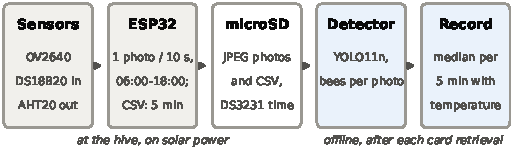
\includegraphics[width=\columnwidth]{assets/architecture.pdf}
  \caption{Processing chain of the station.}
  \label{fig:architecture}
\end{figure}

Fig.~\ref{fig:architecture} shows the processing chain. From 06:00 to 18:00, the board wakes every 10~s, takes one JPEG photo named after the date and time, and sleeps again; every five minutes it appends the time, the three readings, and the battery voltage to a CSV file. After each retrieval, a computer runs the detector on every photo and stores, for each five-minute period, the median number of bees per photo next to the readings of that period.

The detector is the YOLO11n model of the Beehaviour project\footnote{\url{https://github.com/jordicalsinabaldoma/beehavior-upc}, AGPL-3.0.}, trained by its authors on 1756 frames from five of the eight hives of the Sledevi\v{c} and Matuzevi\v{c}ius dataset \cite{sledevic2024dataset}; the other three were kept apart to test it. It has a single class and keeps boxes with confidence above 0.40. The station uses the detection only, with no tracking.

The test uses the 3230 labelled frames of these three hives, called A, B, and C here (\texttt{20230609b}, \texttt{20230711a}, and \texttt{20230711b} in the dataset), reduced to 800 pixels in width. Since the detector never saw them, the test shows how it would do at a new hive, such as the one where the station is installed. A detection is correct when it overlaps a labelled bee with an intersection over union (IoU) of at least 0.5, which gives precision, recall, and F1-score; the count error is the difference between detections and labels in each frame. The agreement is the $R^2$ of the detected count against the line $y=x$, which, unlike the squared correlation, falls with a bias. The alternative method is the background subtraction of Tu et al. \cite{tu2016automatic}: OpenCV's MOG2 learns the empty entrance from consecutive frames, and each foreground region counts as its area divided by that of one bee. Both methods run on the three test videos at ten frames per second and are scored once per second inside the entrance zone, against the hand-labelled tracks with IoU $\geq 0.3$, since a foreground region does not follow the outline of a box. The same tracks, which give the true number of bees in every frame for two minutes per hive, and the frames of hive B, labelled every 0.6~s over 13 minutes of continuous footage (assuming the 50 frames per second of the tracked videos), set the schedule. A two-hour public video of a hive entrance \cite{beecast2021}, without labels, extends the test with the detector counting the bees on the landing board twice per second, since its errors are the same under every schedule.

Next, the labelled frames will be shown as still images on a screen and photographed by the OV2640, with ArUco markers that map the labels onto each photo and identify the frame; the same sequence filmed by a smartphone separates the cost of the screen from that of the camera.

\begin{figure}[t]
  \centering
  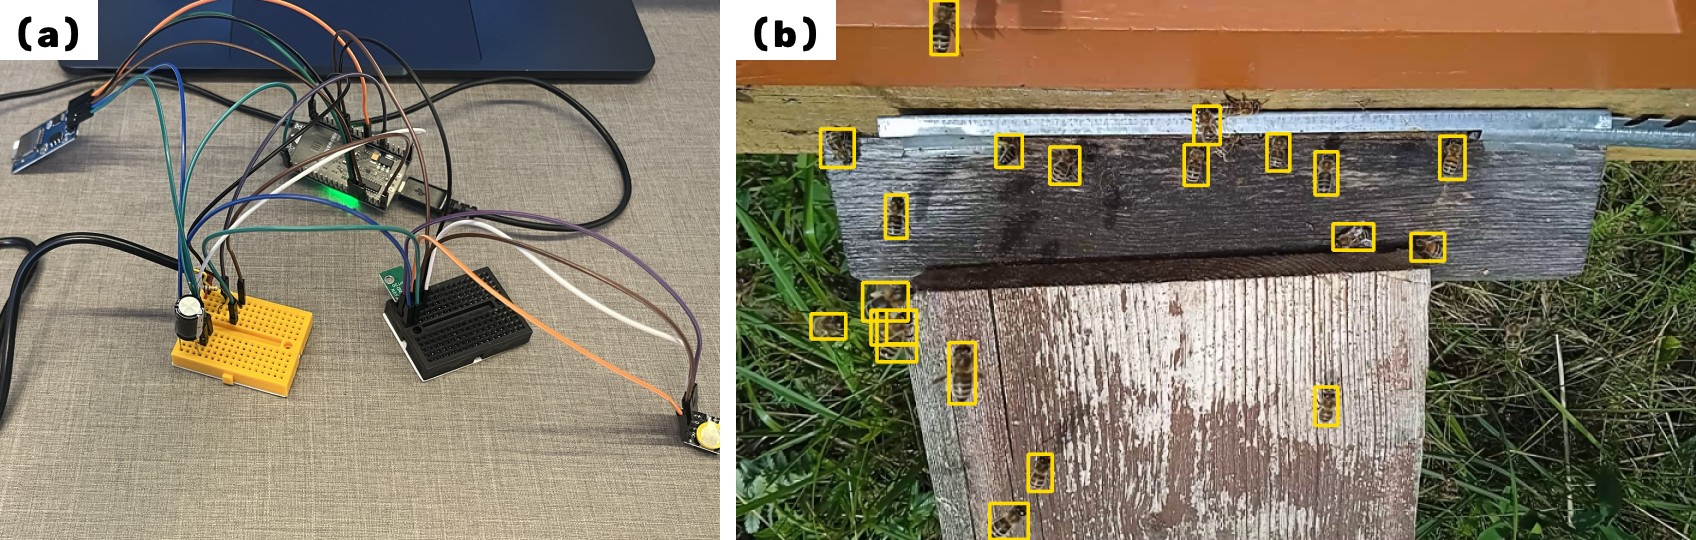
\includegraphics[width=\columnwidth]{assets/prototype-and-detections.jpg}
  \caption{(a) The assembled station: ESP32-WROVER-DEV with the OV2640, microSD reader, DS18B20, AHT20, and DS3231. (b) Detections on a frame of test hive C, at 800 pixels.}
  \label{fig:prototype}
\end{figure}

\section{Results}
\label{sec:results}

The station of Fig.~\ref{fig:prototype}(a) was assembled on two breadboards and powered over USB. Its firmware wakes every 10~s, names each photo after the DS3231 time, appends a CSV row every five minutes, and sleeps again; each start that is not a wake from sleep goes to an event file with its cause, and a watchdog restarts a cycle that exceeds 30~s. With all modules connected, a five-minute test wrote and read back a photo 56 times without a reset, and the clock kept the time on its backup battery with the board unpowered. Side by side, the DS18B20 and the AHT20 read 27.8 and 27.6~$^\circ$C. The solar supply is not built.

\begin{table}[t]
\caption{YOLO11n against the hand labels of the three test hives, at 800 pixels and IoU $\geq 0.5$. Count error: mean absolute difference per frame, with the bias in parentheses and the error relative to the labelled bees.}
\label{tab:detection}
\centering
\footnotesize
\setlength{\tabcolsep}{3pt}
\begin{tabular}{lcccccc}
\hline
Hive & Bees & Prec. & Recall & F1 & Count error & Rel. \\
\hline
A & 6.6 & 0.60 & 0.83 & 0.69 & 2.6 (+2.6) & 40\% \\
B & 19.0 & 0.91 & 0.86 & 0.89 & 1.7 ($-$1.1) & 9\% \\
C & 8.7 & 0.89 & 0.73 & 0.80 & 2.0 ($-$1.6) & 23\% \\
All & 12.3 & 0.83 & 0.83 & 0.83 & 2.1 ($-$0.1) & 17\% \\
\hline
\end{tabular}
\end{table}

Table~\ref{tab:detection} compares the detector with the labels. Over all frames it found 83\% of the bees with a precision of 83\%, and its count was off by 2.1 bees per frame, with an agreement of 0.90. The errors go in opposite directions and depend on the hive. On hive A, with few bees, the detector takes screw heads and objects in the grass for bees, so it overcounts by 2.6 bees, 40\% of the bees present, and the agreement drops to 0.42. Where bees crowd the entrance slot, as in Fig.~\ref{fig:prototype}(b), it misses them: the bias goes from $+1.1$ bees in frames with up to five bees to $-5.5$ in frames with more than 30, which flattens the peaks of activity. A linear correction fitted on two hives raised the error on the third in all three cases, so the bias belongs to each scene and a correction would need labels from the hive where the station is installed.

\begin{table}[t]
\caption{YOLO11n against background subtraction in the entrance zone of the three test videos (358 frames, 13 bees per frame, IoU $\geq 0.3$). Time: per frame on a laptop.}
\label{tab:methods}
\centering
\footnotesize
\setlength{\tabcolsep}{3pt}
\begin{tabular}{lcccccc}
\hline
Method & Prec. & Recall & F1 & Count error & Rel. & Time \\
\hline
YOLO11n & 0.89 & 0.86 & 0.88 & 1.7 ($-$0.5) & 13\% & 19 ms \\
Background sub. & 0.34 & 0.28 & 0.31 & 5.7 ($-$2.4) & 44\% & 7 ms \\
\hline
\end{tabular}
\end{table}

Table~\ref{tab:methods} compares both methods. Background subtraction is faster but misses most bees, because a bee that stands still becomes part of the background: on hive B, where 22\% of the labelled bees are fanning, it undercounted by 8.5 bees per frame. It also needs consecutive frames, which the schedule of single photos does not provide.

On the hand-labelled tracks, the median of a 10~s window changed by half a bee between 50 and one frame per second, so the frame rate does not matter for this count. What matters is how far apart the photos are. On the 13-minute footage, against the median of each 5-minute period, one 10~s burst per period missed by 3 bees, and by up to 7 in one case in ten, while 30 single photos, one every 10~s, missed by half a bee, and by at most 1.5 in nine cases in ten. Against the two-minute tracks, the burst missed by 3 and 4 bees in the two busier hives and the photos by 1. On the two-hour video, where the 5-minute median went from 25 to 61 detected bees, the burst missed by 2 and the photos by half a bee. The station therefore takes one photo every 10~s instead of short bursts. The count measures how many bees are in view, which also rises when bees fan at the entrance in the heat, so it must be read as occupancy of the landing board next to the temperature, not as foraging traffic.

\section{Conclusion}
\label{sec:conclusion}

This work presented a low-cost station, designed for solar power, that records the entrance of a beehive and its temperature on a memory card, without a network, and counts the bees in view offline. On 3230 hand-labelled frames from three test hives the detector never saw, it reached an F1-score of 0.83 and a count error of 2.1 bees per frame. On the test videos, background subtraction reached an F1-score of 0.31 against 0.88 and missed 5.7 bees per frame against 1.7, as it loses the bees that stand still. Its weak points are crowded bees, which it misses, and scene objects, which it adds, with a bias that depends on the hive. Hand-labelled footage and a two-hour public video showed that single photos every 10~s estimate the bees in view better than bursts, with fewer images. The station was assembled and records photos and temperatures on its card with the clock time. The next steps are building the solar supply, measuring the consumption and the autonomy, photographing the labelled frames with the OV2640 to measure the loss caused by the camera, and installing the station at a real hive.

\bibliographystyle{ieeetr}
\bibliography{refs}

\end{document}
